\documentclass{article}
\usepackage{tikz}

\begin{document}
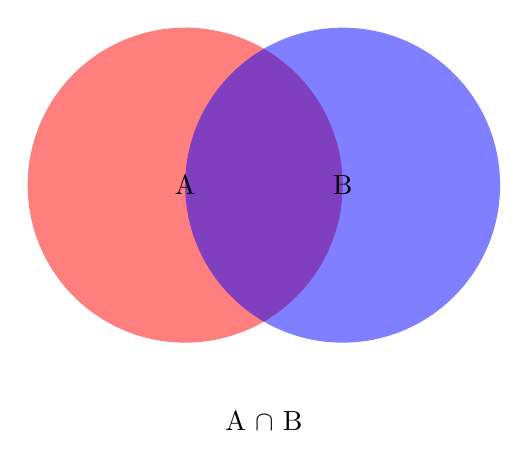
\begin{tikzpicture}
    \begin{scope}[fill opacity=0.5]
    \fill[red] (0,0) circle (2cm);
    \fill[blue] (2cm,0) circle (2cm);
    \end{scope}
    \node at (0,0) {A};
    \node at (2cm,0) {B};
    \node at (1cm,-3cm) {A $\cap$ B};
\end{tikzpicture}
%\end{document}

% \documentclass{article}
% \usepackage{tikz}
% \usetikzlibrary{shapes,backgrounds}

%\begin{document}
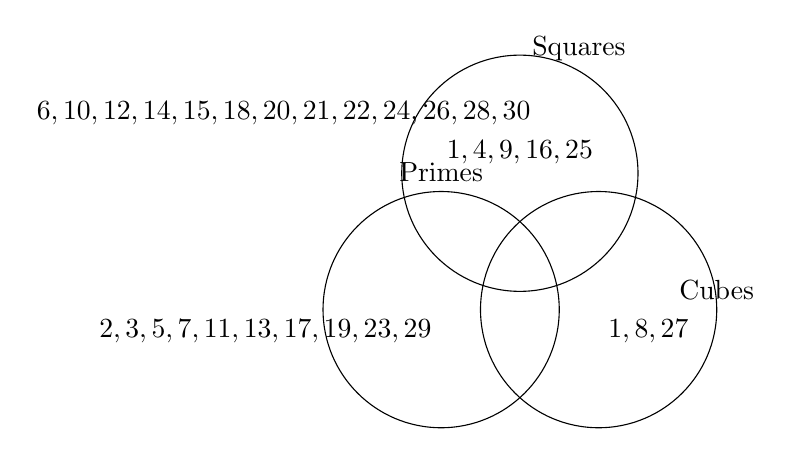
\begin{tikzpicture}
    \def\firstcircle{(0,0) circle (1.5cm)}
    \def\secondcircle{(60:2cm) circle (1.5cm)}
    \def\thirdcircle{(0:2cm) circle (1.5cm)}
    
    % Set A: Prime numbers within 1-30
    \node [above] at (0,1.5) {Primes};
    % Set B: Square numbers within 1-30
    \node [above] at (60:3.5cm) {Squares};
    % Set C: Cube numbers within 1-30
    \node [above] at (0:3.5cm) {Cubes};
    
    \begin{scope}[even odd rule] % for shaded overlapping regions
        \clip \secondcircle;
        \clip \thirdcircle;
    \end{scope}

    \begin{scope}[even odd rule] % for shaded overlapping regions
        \clip \firstcircle;
        \clip \thirdcircle;
    \end{scope}

    \begin{scope}[even odd rule] % for shaded overlapping regions
        \clip \firstcircle;
        \clip \secondcircle;
    \end{scope}
    
    \draw \firstcircle node [below left] {$2,3,5,7,11,13,17,19,23,29$};
    \draw \secondcircle node [above] {$1,4,9,16,25$};
    \draw \thirdcircle node [below right] {$1,8,27$};
    
    % Now place the numbers in the universal set but outside the sets
    \node at (-2, 2.5) {$6,10,12,14,15,18,20,21,22,24,26,28,30$};
    
\end{tikzpicture}

%\documentclass{article}
%\usepackage{tikz}
%\usetikzlibrary{shapes,backgrounds}

%\begin{document}
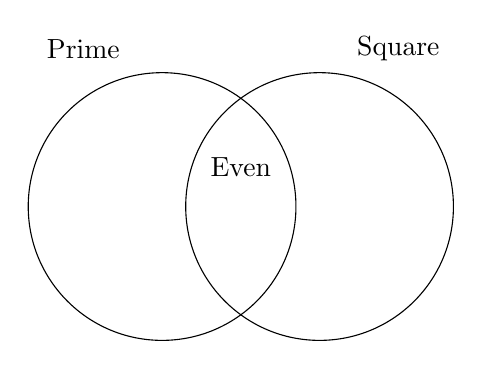
\begin{tikzpicture}
    \node at (-1,2) {Prime}; % Label for the prime set
    \node at (3,2) {Square}; % Label for the square set
    \node at (1,0.5) {Even}; % Label for the even set
    %\node[draw,rectangle] at (1,0.5) {Even}; % Label for the even set

    % Draw the circles for the prime and square sets
    % \draw (0,0) circle (1.5cm);
    \draw (0,0) circle (1.7cm);
    
   % \draw (2,0) circle (1.5cm);
    \draw (2,0) circle (1.7cm);
    

    % You can also add specific elements to each part of the Venn diagram if required
    % For instance, labeling the parts of the Venn diagram could look something like this:
    % \node at (-0.5,-0.5) {2, 3, 5, 7, 11, ...};
    % \node at (2.5,-0.5) {1, 4, 9, 16, 25, ...};
    % \node at (1,-1.5) {Intersection elements, if any};
\end{tikzpicture}

\vspace{20pt}

%\documentclass{article}
%\usepackage{tikz}
%\usetikzlibrary{shapes,backgrounds}

%\begin{document}
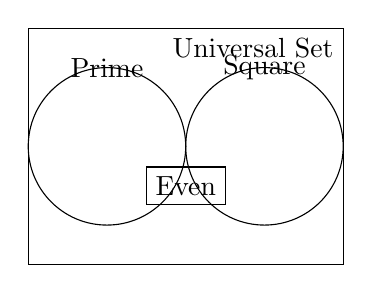
\begin{tikzpicture}
    % Define the bounding box for the universal set
    \draw (0,0) rectangle (4,3);
    \node at (4,3) [below left] {Universal Set};

    % Add labels for each set
    \node at (1,2.5) {Prime};
    \node at (3,2.5) {Square};
    \node[draw,rectangle] at (2,1) {Even};

    % Draw the circles for the prime and square sets
    \draw (1,1.5) circle (1cm);
    \draw (3,1.5) circle (1cm);

    % Optional: Add elements to the sets
    % \node at (1,1.5) {2, 3, 5, 7, ...};
    % \node at (3,1.5) {1, 4, 9, 16, ...};
    % \node at (2,1.5) {Intersection if any};
\end{tikzpicture}

\vspace{20pt}

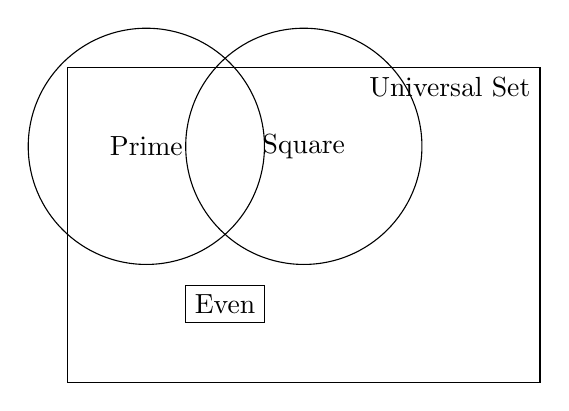
\begin{tikzpicture}
    % Define the bounding box for the universal set
    \draw (0,0) rectangle (6,4);
    \node at (6,4) [below left] {Universal Set};

    % Add labels for each set
    \node at (1,3) {Prime};
    \node at (3,3) {Square};
    \node[draw,rectangle] at (2,1) {Even};

    % Draw the circles for the prime and square sets
    \draw (1,3) circle (1.5cm);
    \draw (3,3) circle (1.5cm);

    % Optional: Add elements to the sets
    % \node at (1,1.5) {2, 3, 5, 7, ...};
    % \node at (3,1.5) {1, 4, 9, 16, ...};
    % \node at (2,1.5) {Intersection if any};
\end{tikzpicture}

\vspace{20pt}

\documentclass{article}
\usepackage{tikz}
\usetikzlibrary{shapes,backgrounds}

\begin{document}
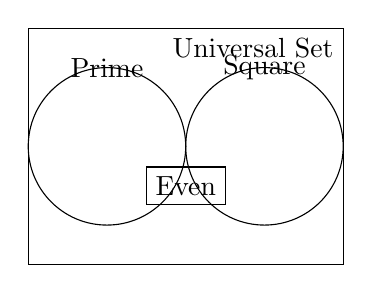
\begin{tikzpicture}
    % Define the bounding box for the universal set
    \draw (0,0) rectangle (4,3);
    \node at (4,3) [below left] {Universal Set};

    % Add labels for each set
    \node at (1,2.5) {Prime};
    \node at (3,2.5) {Square};
    \node[draw,rectangle] at (2,1) {Even};

    % Draw the circles for the prime and square sets
    \draw (1,1.5) circle (1cm);
    \draw (3,1.5) circle (1cm);

    % Optional: Add elements to the sets
    % \node at (1,1.5) {2, 3, 5, 7, ...};
    % \node at (3,1.5) {1, 4, 9, 16, ...};
    % \node at (2,1.5) {Intersection if any};
\end{tikzpicture}

\vspace{10pt}


\item \quad Sort these numbers into the Venn diagram below. Remember, numbers that fit in both circles to be put at the point of intersection (the central oval). Numbers that do not belong to any circle should be put in the sample space (between the rectangle and the circles). 
\[ 2, 3, 4, 5, 7, 9, 10, 11, 12, 13, 14, 15 \]
 \includegraphics[width=10cm]{Year_6_Mixed_Tests/Homework_Tasks/Venn1.png}

\end{document}




\end{document}



 